% =====================================================================
% Borrador de las secciones de Hugo para el informe IEEE de PatrullaIA
% Para pegar en el .tex del equipo. Requiere: graphicx, booktabs, babel (spanish).
%
% ANTES DE ENTREGAR:
%  - [VERIFICAR]: leer Chen, Cheng y Wise (2017) y confirmar o corregir lo marcado.
%  - Las claves de \cite deben coincidir con bibliografia.bib (Deivis).
%  - Las figuras están en outputs/figuras/; ajustar la ruta según dónde esté el .tex.
%  - Confirmar las comisarías de salida con la lista de la PNP.
%  - Completar los [PENDIENTE] con los resultados de Flavia (MLP) y Deivis (GA).
% =====================================================================

\subsection{Investigación 3: rutas de patrullaje sobre la red de calles}
% [VERIFICAR] Revisar título, revista y aportes con el artículo original.
Chen, Cheng y Wise \cite{chen2017} plantean el patrullaje policial como un problema de rutas sobre la red de calles real y no sobre una cuadrícula abstracta. La idea central que tomamos es que la patrulla debe pasar con más frecuencia por los tramos donde se concentra el delito, sin dejar de cubrir el resto del territorio. % [VERIFICAR] caso de estudio (ciudad), método exacto y métricas de evaluación.

De este trabajo adoptamos dos decisiones: (1) representar la ciudad como un grafo de calles obtenido de datos abiertos, y (2) guiar la ruta con un indicador de riesgo por tramo en lugar de la distancia sola. A diferencia de ese trabajo, PatrullaIA calcula una sola ruta por distrito con A* y la compara con BFS, porque el curso pide técnicas de búsqueda clásicas. % [VERIFICAR] que la comparación sea justa con lo que hace el artículo.

\subsection{Módulo de rutas}

\subsubsection{Datos}
Las calles y los lugares se extrajeron del archivo de Perú de OpenStreetMap publicado por Geofabrik (corte del 8 de noviembre de 2026), procesado con la librería \texttt{osmium} y \texttt{osmnx}. Se usaron las calles transitables en auto (filtro \texttt{drive} de \texttt{osmnx}), que en los 43 distritos suman 137\,896 esquinas y 360\,845 tramos dirigidos. Como control, se compararon diez distritos con los datos descargados directamente de la API Overpass: los kilómetros de calle difieren en menos de 1\,\% (9\,890 frente a 9\,910 km) y los lugares en a lo sumo uno por categoría.

\subsubsection{Riesgo de cada calle con descenso del gradiente}
El dataset del MININTER informa las denuncias por distrito, no por calle. Siguiendo el enfoque de \emph{Risk Terrain Modeling} \cite{caplan2011}, se supuso que el delito se concentra cerca de ciertos lugares que sí están en OpenStreetMap. Para cada uno de los 204\,112 tramos (red sin dirección) se contaron los bares, paraderos, mercados, y bancos y cajeros a menos de 100\,m, y se midió la cercanía a la presencia policial más próxima (1 junto a ella y 0 desde 1\,km). El riesgo de un tramo $e$ es
\begin{equation}
  r_e = w_0 + w_1\,\text{bares}_e + w_2\,\text{paraderos}_e + w_3\,\text{mercados}_e + w_4\,\text{cajeros}_e - w_5\,\text{policía}_e ,
\end{equation}
donde $w_0$ es un riesgo base por calle. El alumbrado, previsto en el diseño, se descartó: solo el 1,9\,\% de los tramos de Lima tiene la etiqueta \texttt{lit} (4,6\,\% en Cercado y 3,2\,\% en San Juan de Lurigancho).

Los pesos se ajustaron con descenso del gradiente programado por el equipo, para que la suma del riesgo de las calles de cada distrito se aproxime a su promedio mensual de denuncias de robo y hurto en el periodo de entrenamiento (2018--2024). La pérdida es el error cuadrático medio sobre los 43 distritos; los factores se escalaron por su máximo, el paso se fijó en $1/L$ (con $L$ la constante de Lipschitz del gradiente) y, tras cada paso, los pesos se proyectaron a $w_j \ge 0$ para respetar el signo de cada factor. El resultado coincide con la solución exacta de mínimos cuadrados no negativos (diferencia relativa del orden de $10^{-16}$). La Tabla~\ref{tab:pesos} muestra los pesos.

\begin{table}[htbp]
\caption{Pesos ajustados por descenso del gradiente}
\label{tab:pesos}
\centering
\begin{tabular}{lr}
\toprule
Factor & Peso \\
\midrule
Bancos y cajeros & 0,240 \\
Mercados & 0,177 \\
Paraderos & 0,045 \\
Base por tramo & 0,0015 \\
Bares & 0 \\
Cercanía a la policía & 0 \\
\bottomrule
\end{tabular}
\end{table}

El riesgo se recortó al percentil 99 (2\,205 tramos) y se normalizó entre 0 y 1. Los puntos críticos de cada distrito piloto se eligieron sin \emph{k-means}: se toma la esquina de mayor riesgo y luego la siguiente que esté a más de 300\,m de las ya elegidas, hasta tener ocho (Fig.~\ref{fig:riesgo}).

\begin{figure*}[htbp]
\centering
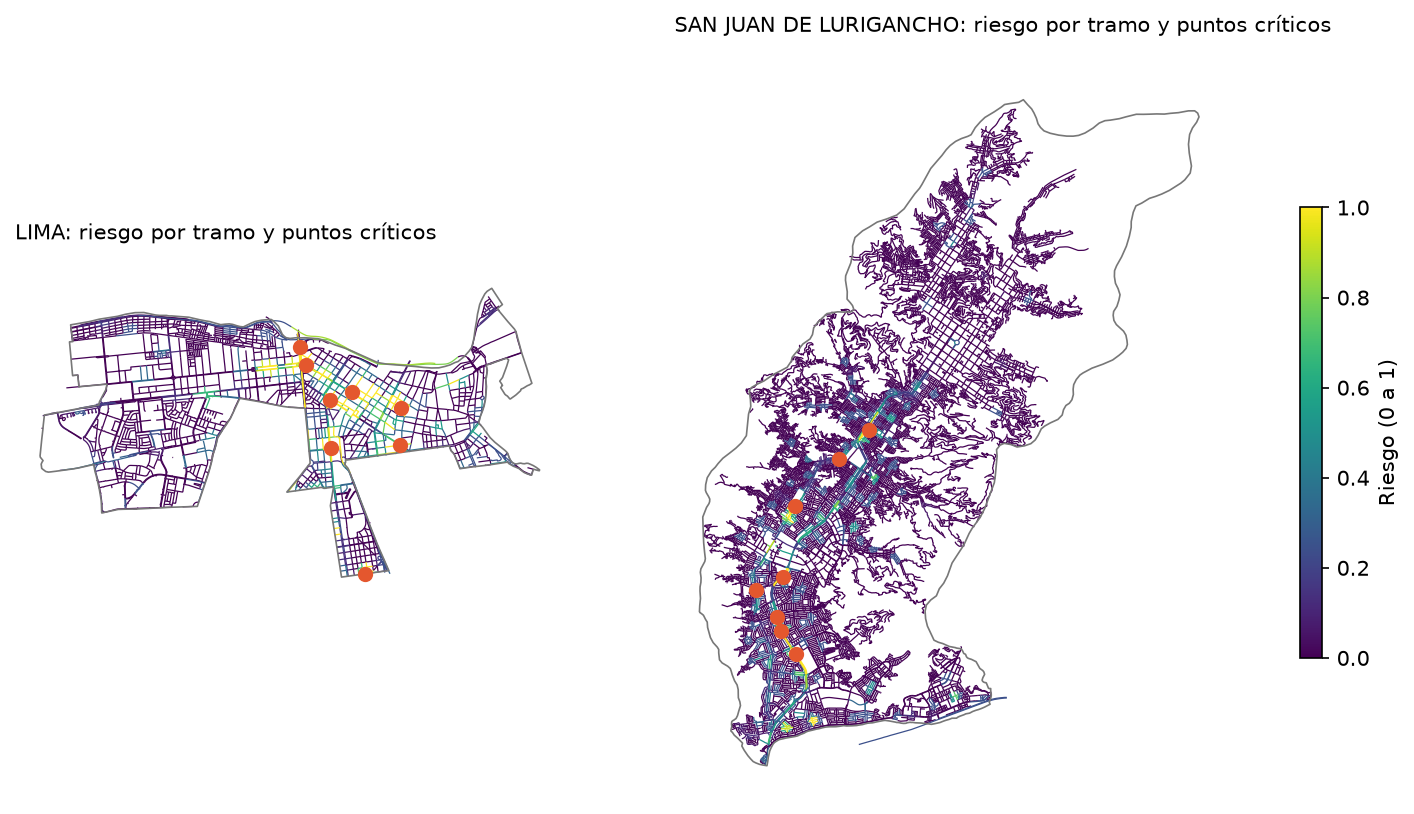
\includegraphics[width=0.9\textwidth]{outputs/figuras/riesgo_pilotos.png}
\caption{Riesgo por tramo (0 a 1) y puntos críticos en Cercado de Lima y San Juan de Lurigancho.}
\label{fig:riesgo}
\end{figure*}

\subsubsection{Ruta con A* y BFS}
Para cada piloto se construyó un grafo dirigido (esquina = nodo, tramo = arista con su largo), que respeta los sentidos únicos y conserva la mayor componente fuertemente conexa: 2\,610 esquinas y 5\,563 tramos en Cercado, y 14\,251 esquinas y 37\,923 tramos en San Juan de Lurigancho. El costo de un tramo es
\begin{equation}
  c(e) = \frac{\ell_e}{1 + \beta\, r_e},
\end{equation}
de modo que una calle riesgosa cuesta menos y la patrulla tiende a pasar por ella; con $\beta = 0$ se obtiene la ruta más corta. La heurística de A* es $h(n) = d(n, \text{meta})/(1+\beta)$, con $d$ la distancia sobre la superficie terrestre, la misma fórmula con la que se mide el largo de las calles. Como $r_e \in [0,1]$ y ningún tramo es más corto que la recta entre sus extremos, $h$ es admisible y consistente, y A* devuelve la ruta óptima. Se comprobó numéricamente que A* da el mismo costo que \texttt{networkx} y que $h$ no sobreestima el costo real en ninguno de los nodos de Cercado.

BFS se usó para verificar que, desde la comisaría, se alcanzan todos los puntos críticos y se puede volver. La patrulla sale de la comisaría más cercana al centro de los puntos críticos (Comisaría PNP Cotabambas en Cercado y Comisaría PNP Canto Rey en San Juan de Lurigancho; se excluyeron las comisarías de la familia, que no patrullan). % [VERIFICAR] con la lista de la PNP.
Con ocho puntos se probaron los $8! = 40\,320$ órdenes de visita sobre la matriz de costos calculada con A*, y se eligió el de menor costo total de ida y vuelta (Fig.~\ref{fig:rutas}).

\begin{figure*}[htbp]
\centering
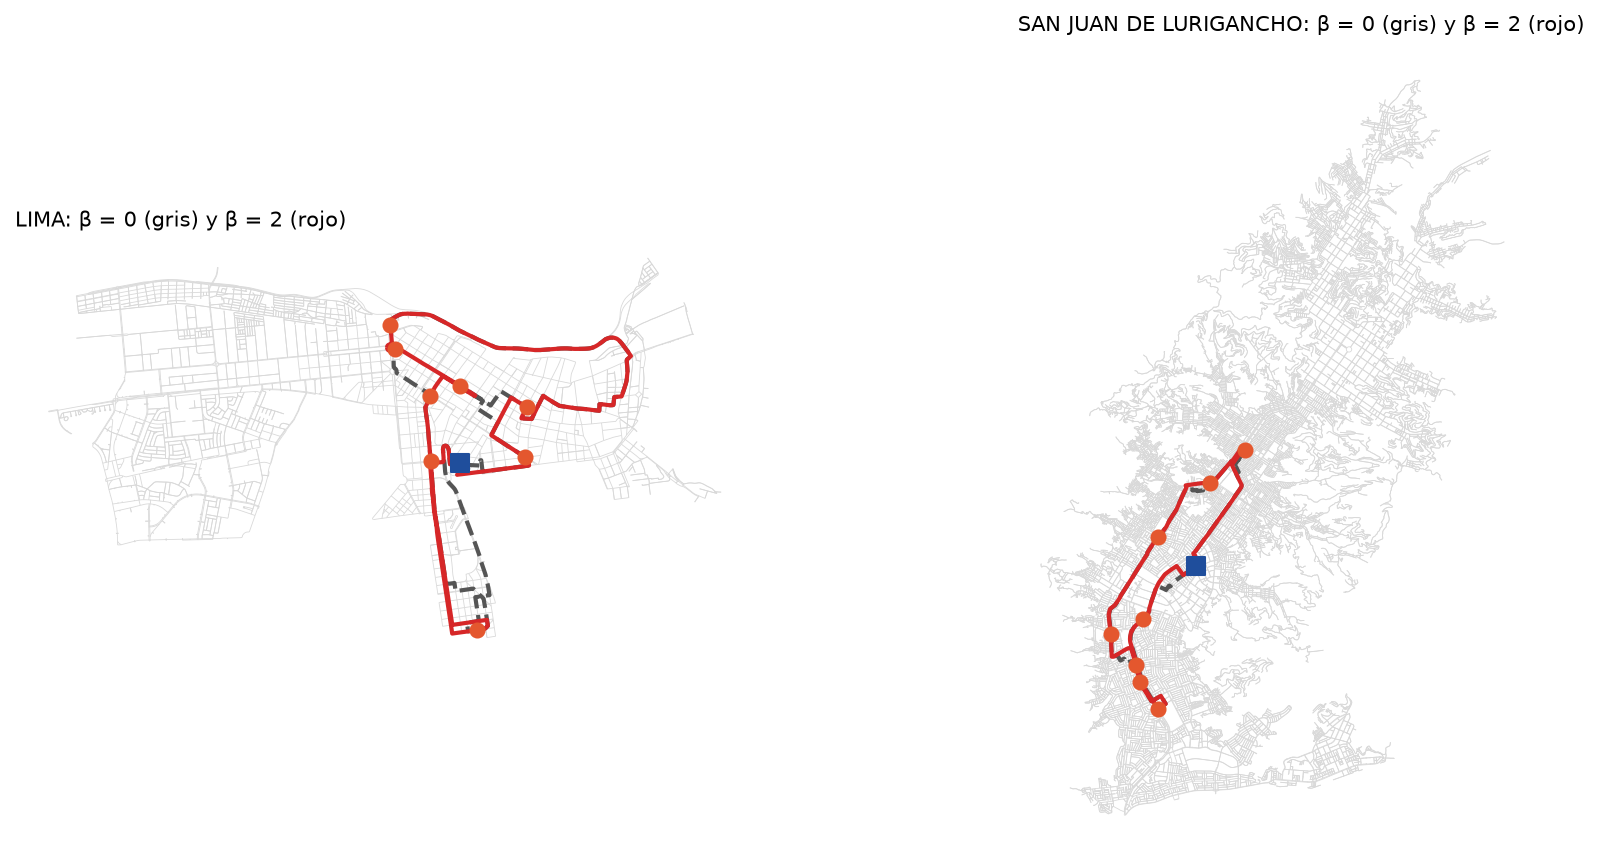
\includegraphics[width=0.9\textwidth]{outputs/figuras/rutas_pilotos.png}
\caption{Ruta más corta ($\beta=0$, gris) y ruta guiada por el riesgo ($\beta=2$, rojo). Cuadrado: comisaría de salida; círculos: puntos críticos.}
\label{fig:rutas}
\end{figure*}

\subsection{Evaluación y ética}

\subsubsection{Riesgo por calle}
Para saber si los lugares de OpenStreetMap explican las denuncias más allá del tamaño del distrito, se validó dejando un distrito fuera (43 ajustes). Se comparó con un modelo base que solo usa la cantidad de tramos (Tabla~\ref{tab:loo}). El modelo con lugares reduce el error porcentual de 160\,\% a 46\,\%.

\begin{table}[htbp]
\caption{Validación dejando un distrito fuera (denuncias por mes)}
\label{tab:loo}
\centering
\begin{tabular}{lrrr}
\toprule
Modelo & MAE & MAPE (\%) & $R^2$ \\
\midrule
Solo cantidad de tramos & 132,1 & 159,8 & 0,19 \\
Con lugares de OSM & 76,5 & 45,9 & 0,63 \\
\bottomrule
\end{tabular}
\end{table}

\subsubsection{Rutas}
La Tabla~\ref{tab:beta} muestra el efecto de $\beta$. En San Juan de Lurigancho, pasar de $\beta=0$ a $\beta=2$ sube la parte del recorrido que va por calles de riesgo mayor a 0,5 de 33\,\% a 46\,\%, con una ruta solo 3\,\% más larga.

\begin{table}[htbp]
\caption{Efecto de $\beta$ en la ruta completa}
\label{tab:beta}
\centering
\begin{tabular}{lcrrr}
\toprule
Distrito & $\beta$ & km & Riesgo medio & \% km riesgo $>0{,}5$ \\
\midrule
Cercado & 0 & 19,3 & 0,47 & 50,2 \\
Cercado & 2 & 19,6 & 0,52 & 54,2 \\
S. J. de Lurigancho & 0 & 18,3 & 0,44 & 33,3 \\
S. J. de Lurigancho & 2 & 18,9 & 0,52 & 45,7 \\
\bottomrule
\end{tabular}
\end{table}

La Tabla~\ref{tab:busqueda} compara los algoritmos sobre todos los tramos del recorrido con $\beta=2$. Gracias a la heurística, A* revisa 46\,\% menos nodos que Dijkstra (A* con $h=0$) en Cercado y 68\,\% menos en San Juan de Lurigancho, con el mismo resultado. BFS es rápido, pero minimiza la cantidad de tramos y no la distancia ni el riesgo: su recorrido es 1,4\,\% más largo en Cercado y 17\,\% en San Juan de Lurigancho.

\begin{table}[htbp]
\caption{A*, Dijkstra y BFS en el recorrido completo ($\beta=2$)}
\label{tab:busqueda}
\centering
\begin{tabular}{llrrr}
\toprule
Distrito & Algoritmo & Nodos & ms & Metros \\
\midrule
Cercado & A* & 1\,267 & 6,9 & 19\,603 \\
 & Dijkstra & 2\,332 & 9,1 & 19\,603 \\
 & BFS & 2\,627 & 3,5 & 19\,885 \\
\midrule
S. J. de Lurigancho & A* & 3\,633 & 23,0 & 18\,854 \\
 & Dijkstra & 11\,506 & 56,4 & 18\,854 \\
 & BFS & 13\,255 & 21,4 & 22\,031 \\
\bottomrule
\end{tabular}
\end{table}

% [PENDIENTE] Predicción (Flavia): MAE, RMSE y MAPE del ingenuo, el perceptrón y la MLP en el conjunto de prueba (ene--jul 2026).
% [PENDIENTE] Asignación (Deivis): utilidad del GA frente al reparto parejo, el proporcional y el actual (RENAMU).

\subsubsection{Limitaciones}
\begin{itemize}
  \item Los pesos se calibran con solo 43 distritos: son orientativos, no causales.
  \item OpenStreetMap está incompleto en Lima: registra solo 316 bares en toda la provincia y casi no tiene alumbrado. Por eso los bares quedaron con peso 0 y el alumbrado se descartó.
  \item La cercanía a la policía no restó riesgo (peso 0), probablemente porque la policía se ubica donde hay más delito; con datos agregados no se puede separar ese efecto.
  \item Las rutas no consideran el tráfico vehicular ni la hora del día, que OpenStreetMap no registra.
  \item Las comisarías provienen de OpenStreetMap y deben verificarse con la lista oficial de la PNP.
\end{itemize}

\subsubsection{Ética}
Las denuncias miden dónde la gente denuncia, no exactamente dónde ocurre el delito: los distritos o grupos que denuncian menos quedan subrepresentados. Además, existe un riesgo de retroalimentación: si se patrulla más donde el modelo indica, se registran más denuncias allí y el modelo refuerza su propia predicción. Por eso PatrullaIA debe usarse como apoyo a la decisión, revisarse periódicamente y no aplicarse sobre personas: un riesgo alto marca una calle para patrullar, no a quienes viven o transitan por ella. Los datos usados son agregados por distrito y mes, y no contienen información personal.
